\documentclass[twoside]{book}

% Packages required by doxygen
\usepackage{fixltx2e}
\usepackage{calc}
\usepackage{doxygen}
\usepackage[export]{adjustbox} % also loads graphicx
\usepackage{graphicx}
\usepackage[utf8]{inputenc}
\usepackage{makeidx}
\usepackage{multicol}
\usepackage{multirow}
\PassOptionsToPackage{warn}{textcomp}
\usepackage{textcomp}
\usepackage[nointegrals]{wasysym}
\usepackage[table]{xcolor}

% Font selection
\usepackage[T1]{fontenc}
\usepackage[scaled=.90]{helvet}
\usepackage{courier}
\usepackage{amssymb}
\usepackage{sectsty}
\renewcommand{\familydefault}{\sfdefault}
\allsectionsfont{%
  \fontseries{bc}\selectfont%
  \color{darkgray}%
}
\renewcommand{\DoxyLabelFont}{%
  \fontseries{bc}\selectfont%
  \color{darkgray}%
}
\newcommand{\+}{\discretionary{\mbox{\scriptsize$\hookleftarrow$}}{}{}}

% Page & text layout
\usepackage{geometry}
\geometry{%
  a4paper,%
  top=2.5cm,%
  bottom=2.5cm,%
  left=2.5cm,%
  right=2.5cm%
}
\tolerance=750
\hfuzz=15pt
\hbadness=750
\setlength{\emergencystretch}{15pt}
\setlength{\parindent}{0cm}
\setlength{\parskip}{3ex plus 2ex minus 2ex}
\makeatletter
\renewcommand{\paragraph}{%
  \@startsection{paragraph}{4}{0ex}{-1.0ex}{1.0ex}{%
    \normalfont\normalsize\bfseries\SS@parafont%
  }%
}
\renewcommand{\subparagraph}{%
  \@startsection{subparagraph}{5}{0ex}{-1.0ex}{1.0ex}{%
    \normalfont\normalsize\bfseries\SS@subparafont%
  }%
}
\makeatother

% Headers & footers
\usepackage{fancyhdr}
\pagestyle{fancyplain}
\fancyhead[LE]{\fancyplain{}{\bfseries\thepage}}
\fancyhead[CE]{\fancyplain{}{}}
\fancyhead[RE]{\fancyplain{}{\bfseries\leftmark}}
\fancyhead[LO]{\fancyplain{}{\bfseries\rightmark}}
\fancyhead[CO]{\fancyplain{}{}}
\fancyhead[RO]{\fancyplain{}{\bfseries\thepage}}
\fancyfoot[LE]{\fancyplain{}{}}
\fancyfoot[CE]{\fancyplain{}{}}
\fancyfoot[RE]{\fancyplain{}{\bfseries\scriptsize Generated by Doxygen }}
\fancyfoot[LO]{\fancyplain{}{\bfseries\scriptsize Generated by Doxygen }}
\fancyfoot[CO]{\fancyplain{}{}}
\fancyfoot[RO]{\fancyplain{}{}}
\renewcommand{\footrulewidth}{0.4pt}
\renewcommand{\chaptermark}[1]{%
  \markboth{#1}{}%
}
\renewcommand{\sectionmark}[1]{%
  \markright{\thesection\ #1}%
}

% Indices & bibliography
\usepackage{natbib}
\usepackage[titles]{tocloft}
\setcounter{tocdepth}{3}
\setcounter{secnumdepth}{5}
\makeindex

% Hyperlinks (required, but should be loaded last)
\usepackage{ifpdf}
\ifpdf
  \usepackage[pdftex,pagebackref=true]{hyperref}
\else
  \usepackage[ps2pdf,pagebackref=true]{hyperref}
\fi
\hypersetup{%
  colorlinks=true,%
  linkcolor=blue,%
  citecolor=blue,%
  unicode%
}

% Custom commands
\newcommand{\clearemptydoublepage}{%
  \newpage{\pagestyle{empty}\cleardoublepage}%
}

\usepackage{caption}
\captionsetup{labelsep=space,justification=centering,font={bf},singlelinecheck=off,skip=4pt,position=top}

%===== C O N T E N T S =====

\begin{document}

% Titlepage & ToC
\hypersetup{pageanchor=false,
             bookmarksnumbered=true,
             pdfencoding=unicode
            }
\pagenumbering{alph}
\begin{titlepage}
\vspace*{7cm}
\begin{center}%
{\Large cpplibs }\\
\vspace*{1cm}
{\large Generated by Doxygen 1.8.13}\\
\end{center}
\end{titlepage}
\clearemptydoublepage
\pagenumbering{roman}
\tableofcontents
\clearemptydoublepage
\pagenumbering{arabic}
\hypersetup{pageanchor=true}

%--- Begin generated contents ---
\chapter{Cpp\+Libs}
\label{md_README}
\Hypertarget{md_README}
\subsection*{T\+O\+DO}


\begin{DoxyItemize}
\item input stream and output stream separate closable (?)
\end{DoxyItemize}

\subsection*{Build}

run ./configure make -\/C build

\subsection*{Documentation}

available\+: \href{https://devfix.github.io/cpplibs/html/index.html}{\tt here} 
\chapter{Hierarchical Index}
\section{Class Hierarchy}
This inheritance list is sorted roughly, but not completely, alphabetically\+:\begin{DoxyCompactList}
\item exception\begin{DoxyCompactList}
\item \contentsline{section}{devfix\+:\+:base\+:\+:error\+:\+:baseexception}{\pageref{structdevfix_1_1base_1_1error_1_1baseexception}}{}
\begin{DoxyCompactList}
\item \contentsline{section}{devfix\+:\+:base\+:\+:error\+:\+:interruptedexception}{\pageref{structdevfix_1_1base_1_1error_1_1interruptedexception}}{}
\item \contentsline{section}{devfix\+:\+:base\+:\+:error\+:\+:ioexception}{\pageref{structdevfix_1_1base_1_1error_1_1ioexception}}{}
\item \contentsline{section}{devfix\+:\+:base\+:\+:error\+:\+:timeoutexception}{\pageref{structdevfix_1_1base_1_1error_1_1timeoutexception}}{}
\item \contentsline{section}{devfix\+:\+:net\+:\+:socketexception}{\pageref{structdevfix_1_1net_1_1socketexception}}{}
\end{DoxyCompactList}
\end{DoxyCompactList}
\item \contentsline{section}{devfix\+:\+:net\+:\+:inetaddress}{\pageref{structdevfix_1_1net_1_1inetaddress}}{}
\item \contentsline{section}{devfix\+:\+:base\+:\+:io\+:\+:inputstream}{\pageref{structdevfix_1_1base_1_1io_1_1inputstream}}{}
\begin{DoxyCompactList}
\item \contentsline{section}{devfix\+:\+:base\+:\+:io\+:\+:source}{\pageref{structdevfix_1_1base_1_1io_1_1source}}{}
\end{DoxyCompactList}
\item \contentsline{section}{devfix\+:\+:net\+:\+:netbuilder}{\pageref{structdevfix_1_1net_1_1netbuilder}}{}
\item \contentsline{section}{devfix\+:\+:base\+:\+:io\+:\+:outputstream}{\pageref{structdevfix_1_1base_1_1io_1_1outputstream}}{}
\begin{DoxyCompactList}
\item \contentsline{section}{devfix\+:\+:base\+:\+:io\+:\+:sink}{\pageref{structdevfix_1_1base_1_1io_1_1sink}}{}
\end{DoxyCompactList}
\item \contentsline{section}{devfix\+:\+:net\+:\+:serversocket}{\pageref{structdevfix_1_1net_1_1serversocket}}{}
\item \contentsline{section}{devfix\+:\+:net\+:\+:socket}{\pageref{structdevfix_1_1net_1_1socket}}{}
\end{DoxyCompactList}

\chapter{Class Index}
\section{Class List}
Here are the classes, structs, unions and interfaces with brief descriptions\+:\begin{DoxyCompactList}
\item\contentsline{section}{\hyperlink{structdevfix_1_1base_1_1error_1_1baseexception}{devfix\+::base\+::error\+::baseexception} \\*Abstract error base class }{\pageref{structdevfix_1_1base_1_1error_1_1baseexception}}{}
\item\contentsline{section}{\hyperlink{structdevfix_1_1net_1_1inetaddress}{devfix\+::net\+::inetaddress} }{\pageref{structdevfix_1_1net_1_1inetaddress}}{}
\item\contentsline{section}{\hyperlink{structdevfix_1_1base_1_1io_1_1inputstream}{devfix\+::base\+::io\+::inputstream} \\*Superclass of all classes representing an input stream of bytes }{\pageref{structdevfix_1_1base_1_1io_1_1inputstream}}{}
\item\contentsline{section}{\hyperlink{structdevfix_1_1base_1_1error_1_1interruptedexception}{devfix\+::base\+::error\+::interruptedexception} \\*Thrown when an operation is interrupted, either before or during the activity }{\pageref{structdevfix_1_1base_1_1error_1_1interruptedexception}}{}
\item\contentsline{section}{\hyperlink{structdevfix_1_1base_1_1error_1_1ioexception}{devfix\+::base\+::error\+::ioexception} \\*Signals that an I/O error of some sort has occurred }{\pageref{structdevfix_1_1base_1_1error_1_1ioexception}}{}
\item\contentsline{section}{\hyperlink{structdevfix_1_1net_1_1netbuilder}{devfix\+::net\+::netbuilder} }{\pageref{structdevfix_1_1net_1_1netbuilder}}{}
\item\contentsline{section}{\hyperlink{structdevfix_1_1base_1_1io_1_1outputstream}{devfix\+::base\+::io\+::outputstream} \\*Superclass of all classes representing an output stream of bytes }{\pageref{structdevfix_1_1base_1_1io_1_1outputstream}}{}
\item\contentsline{section}{\hyperlink{structdevfix_1_1net_1_1serversocket}{devfix\+::net\+::serversocket} }{\pageref{structdevfix_1_1net_1_1serversocket}}{}
\item\contentsline{section}{\hyperlink{structdevfix_1_1base_1_1io_1_1sink}{devfix\+::base\+::io\+::sink} }{\pageref{structdevfix_1_1base_1_1io_1_1sink}}{}
\item\contentsline{section}{\hyperlink{structdevfix_1_1net_1_1socket}{devfix\+::net\+::socket} }{\pageref{structdevfix_1_1net_1_1socket}}{}
\item\contentsline{section}{\hyperlink{structdevfix_1_1net_1_1socketexception}{devfix\+::net\+::socketexception} \\*Thrown to indicate that there is an error creating or accessing a Socket }{\pageref{structdevfix_1_1net_1_1socketexception}}{}
\item\contentsline{section}{\hyperlink{structdevfix_1_1base_1_1io_1_1source}{devfix\+::base\+::io\+::source} }{\pageref{structdevfix_1_1base_1_1io_1_1source}}{}
\item\contentsline{section}{\hyperlink{structdevfix_1_1base_1_1error_1_1timeoutexception}{devfix\+::base\+::error\+::timeoutexception} \\*Exception thrown when a blocking operation times out }{\pageref{structdevfix_1_1base_1_1error_1_1timeoutexception}}{}
\end{DoxyCompactList}

\chapter{Class Documentation}
\hypertarget{uniondevfix_1_1net_1_1inetaddress_1_1address}{}\section{devfix\+:\+:net\+:\+:inetaddress\+:\+:address Union Reference}
\label{uniondevfix_1_1net_1_1inetaddress_1_1address}\index{devfix\+::net\+::inetaddress\+::address@{devfix\+::net\+::inetaddress\+::address}}
\subsection*{Public Attributes}
\begin{DoxyCompactItemize}
\item 
\mbox{\Hypertarget{uniondevfix_1_1net_1_1inetaddress_1_1address_a4b43c8addd428389334ecc90eda802d0}\label{uniondevfix_1_1net_1_1inetaddress_1_1address_a4b43c8addd428389334ecc90eda802d0}} 
std\+::uint32\+\_\+t {\bfseries s\+\_\+addr}
\item 
\mbox{\Hypertarget{uniondevfix_1_1net_1_1inetaddress_1_1address_a4dec3bb1439fd98072f89f7685c177a2}\label{uniondevfix_1_1net_1_1inetaddress_1_1address_a4dec3bb1439fd98072f89f7685c177a2}} 
char {\bfseries s\+\_\+bytes} \mbox{[}4\mbox{]}
\end{DoxyCompactItemize}


The documentation for this union was generated from the following file\+:\begin{DoxyCompactItemize}
\item 
devfix/net/inetaddress.\+h\end{DoxyCompactItemize}

\hypertarget{unionaddress}{}\section{address Union Reference}
\label{unionaddress}\index{address@{address}}
\subsection*{Public Attributes}
\begin{DoxyCompactItemize}
\item 
\mbox{\Hypertarget{unionaddress_a2bebc42b2bcf9bec5d48178d60f049c7}\label{unionaddress_a2bebc42b2bcf9bec5d48178d60f049c7}} 
std\+::uint32\+\_\+t {\bfseries s\+\_\+addr}
\item 
\mbox{\Hypertarget{unionaddress_a3a6b414db00db509860c8537da888e24}\label{unionaddress_a3a6b414db00db509860c8537da888e24}} 
char {\bfseries s\+\_\+bytes} \mbox{[}4\mbox{]}
\end{DoxyCompactItemize}


The documentation for this union was generated from the following file\+:\begin{DoxyCompactItemize}
\item 
devfix/net/inetaddress.\+h\end{DoxyCompactItemize}

\hypertarget{structdevfix_1_1base_1_1exception}{}\section{devfix\+:\+:base\+:\+:exception Struct Reference}
\label{structdevfix_1_1base_1_1exception}\index{devfix\+::base\+::exception@{devfix\+::base\+::exception}}


{\ttfamily \#include $<$exception.\+h$>$}



Inheritance diagram for devfix\+:\+:base\+:\+:exception\+:

\hypertarget{structdevfix_1_1net_1_1inetaddress}{}\section{devfix\+:\+:net\+:\+:inetaddress Struct Reference}
\label{structdevfix_1_1net_1_1inetaddress}\index{devfix\+::net\+::inetaddress@{devfix\+::net\+::inetaddress}}


Collaboration diagram for devfix\+:\+:net\+:\+:inetaddress\+:
% FIG 0
\subsection*{Classes}
\begin{DoxyCompactItemize}
\item 
union \hyperlink{uniondevfix_1_1net_1_1inetaddress_1_1address}{address}
\end{DoxyCompactItemize}
\subsection*{Public Types}
\begin{DoxyCompactItemize}
\item 
\mbox{\Hypertarget{structdevfix_1_1net_1_1inetaddress_a31ec66f69260c75bfa5105d8e042ff06}\label{structdevfix_1_1net_1_1inetaddress_a31ec66f69260c75bfa5105d8e042ff06}} 
enum {\bfseries family} \+: char \{ {\bfseries U\+N\+S\+U\+P\+P\+O\+R\+T\+ED} = 0, 
{\bfseries I\+P\+V4} = 1
 \}
\item 
\mbox{\Hypertarget{structdevfix_1_1net_1_1inetaddress_a3eaadc730f2b4625987cf948ea485410}\label{structdevfix_1_1net_1_1inetaddress_a3eaadc730f2b4625987cf948ea485410}} 
typedef std\+::uint16\+\_\+t {\bfseries port\+\_\+t}
\end{DoxyCompactItemize}
\subsection*{Public Member Functions}
\begin{DoxyCompactItemize}
\item 
\mbox{\Hypertarget{structdevfix_1_1net_1_1inetaddress_a4524692fae7a767e38600012c6f8f3cf}\label{structdevfix_1_1net_1_1inetaddress_a4524692fae7a767e38600012c6f8f3cf}} 
std\+::string {\bfseries get\+\_\+host} () const noexcept
\end{DoxyCompactItemize}
\subsection*{Static Public Member Functions}
\begin{DoxyCompactItemize}
\item 
\mbox{\Hypertarget{structdevfix_1_1net_1_1inetaddress_a1805a7f56b3c4313232293580b052c7c}\label{structdevfix_1_1net_1_1inetaddress_a1805a7f56b3c4313232293580b052c7c}} 
static \hyperlink{structdevfix_1_1net_1_1inetaddress}{inetaddress} {\bfseries create\+\_\+by\+\_\+host} (const std\+::string \&host, port\+\_\+t port, family family=family\+::\+I\+P\+V4)
\end{DoxyCompactItemize}
\subsection*{Public Attributes}
\begin{DoxyCompactItemize}
\item 
\mbox{\Hypertarget{structdevfix_1_1net_1_1inetaddress_a3752ca3c3b6522ec4e1777287627cbe3}\label{structdevfix_1_1net_1_1inetaddress_a3752ca3c3b6522ec4e1777287627cbe3}} 
enum devfix\+::net\+::inetaddress\+::family {\bfseries \+\_\+\+\_\+attribute\+\_\+\+\_\+}
\item 
\mbox{\Hypertarget{structdevfix_1_1net_1_1inetaddress_a902c9b8140f7c1fad452ef9de7f86561}\label{structdevfix_1_1net_1_1inetaddress_a902c9b8140f7c1fad452ef9de7f86561}} 
\hyperlink{uniondevfix_1_1net_1_1inetaddress_1_1address}{address} {\bfseries address\+\_\+} = \{0\}
\item 
\mbox{\Hypertarget{structdevfix_1_1net_1_1inetaddress_a3b666575020939365ebcec1d7aeb0f34}\label{structdevfix_1_1net_1_1inetaddress_a3b666575020939365ebcec1d7aeb0f34}} 
port\+\_\+t {\bfseries port\+\_\+} = 0
\item 
\mbox{\Hypertarget{structdevfix_1_1net_1_1inetaddress_af025a2c8b37c28f5553f6f0c350d3765}\label{structdevfix_1_1net_1_1inetaddress_af025a2c8b37c28f5553f6f0c350d3765}} 
family {\bfseries family\+\_\+} = family\+::\+U\+N\+S\+U\+P\+P\+O\+R\+T\+ED
\end{DoxyCompactItemize}


The documentation for this struct was generated from the following files\+:\begin{DoxyCompactItemize}
\item 
devfix/net/inetaddress.\+h\item 
devfix/net/inetaddress.\+cpp\end{DoxyCompactItemize}

\hypertarget{structdevfix_1_1base_1_1interruptedexception}{}\section{devfix\+:\+:base\+:\+:interruptedexception Struct Reference}
\label{structdevfix_1_1base_1_1interruptedexception}\index{devfix\+::base\+::interruptedexception@{devfix\+::base\+::interruptedexception}}


{\ttfamily \#include $<$interruptedexception.\+h$>$}



Inheritance diagram for devfix\+:\+:base\+:\+:interruptedexception\+:
% FIG 0


Collaboration diagram for devfix\+:\+:base\+:\+:interruptedexception\+:
% FIG 1
\subsection*{Public Member Functions}
\begin{DoxyCompactItemize}
\item 
\hyperlink{structdevfix_1_1base_1_1interruptedexception_ac7860de3d6456588f4afb1cb5b517ff5}{interruptedexception} (const std\+::string \&what\+\_\+arg, int err=-\/1)
\item 
\hyperlink{structdevfix_1_1base_1_1interruptedexception_a3115c6a0ad2a463d04629df99ec4d119}{interruptedexception} (const char $\ast$what\+\_\+arg, int err=-\/1)
\end{DoxyCompactItemize}
\subsection*{Additional Inherited Members}


\subsection{Detailed Description}
Exception for interruptions. 
\begin{DoxyTemplParams}{Template Parameters}
{\em T} & Type of character \\
\hline
\end{DoxyTemplParams}


\subsection{Constructor \& Destructor Documentation}
\mbox{\Hypertarget{structdevfix_1_1base_1_1interruptedexception_ac7860de3d6456588f4afb1cb5b517ff5}\label{structdevfix_1_1base_1_1interruptedexception_ac7860de3d6456588f4afb1cb5b517ff5}} 
\index{devfix\+::base\+::interruptedexception@{devfix\+::base\+::interruptedexception}!interruptedexception@{interruptedexception}}
\index{interruptedexception@{interruptedexception}!devfix\+::base\+::interruptedexception@{devfix\+::base\+::interruptedexception}}
\subsubsection{\texorpdfstring{interruptedexception()}{interruptedexception()}\hspace{0.1cm}{\footnotesize\ttfamily [1/2]}}
{\footnotesize\ttfamily devfix\+::base\+::interruptedexception\+::interruptedexception (\begin{DoxyParamCaption}\item[{const std\+::string \&}]{what\+\_\+arg,  }\item[{int}]{err = {\ttfamily -\/1} }\end{DoxyParamCaption})\hspace{0.3cm}{\ttfamily [inline]}, {\ttfamily [explicit]}}

Constructs the exception object with what\+\_\+arg as explanatory std\+::string that can be accessed through \hyperlink{structdevfix_1_1base_1_1exception_ad2066a6a81737c0fdf776120a6ca69d2}{what()}. 
\begin{DoxyParams}{Parameters}
{\em what\+\_\+arg} & description \\
\hline
\end{DoxyParams}
\mbox{\Hypertarget{structdevfix_1_1base_1_1interruptedexception_a3115c6a0ad2a463d04629df99ec4d119}\label{structdevfix_1_1base_1_1interruptedexception_a3115c6a0ad2a463d04629df99ec4d119}} 
\index{devfix\+::base\+::interruptedexception@{devfix\+::base\+::interruptedexception}!interruptedexception@{interruptedexception}}
\index{interruptedexception@{interruptedexception}!devfix\+::base\+::interruptedexception@{devfix\+::base\+::interruptedexception}}
\subsubsection{\texorpdfstring{interruptedexception()}{interruptedexception()}\hspace{0.1cm}{\footnotesize\ttfamily [2/2]}}
{\footnotesize\ttfamily devfix\+::base\+::interruptedexception\+::interruptedexception (\begin{DoxyParamCaption}\item[{const char $\ast$}]{what\+\_\+arg,  }\item[{int}]{err = {\ttfamily -\/1} }\end{DoxyParamCaption})\hspace{0.3cm}{\ttfamily [inline]}, {\ttfamily [explicit]}}

Constructs the exception object with what\+\_\+arg as explanatory c-\/string that can be accessed through \hyperlink{structdevfix_1_1base_1_1exception_ad2066a6a81737c0fdf776120a6ca69d2}{what()}. 
\begin{DoxyParams}{Parameters}
{\em what\+\_\+arg} & description \\
\hline
\end{DoxyParams}


The documentation for this struct was generated from the following file\+:\begin{DoxyCompactItemize}
\item 
devfix/base/interruptedexception.\+h\end{DoxyCompactItemize}

\hypertarget{structdevfix_1_1net_1_1netbuilder}{}\section{devfix\+:\+:net\+:\+:netbuilder Struct Reference}
\label{structdevfix_1_1net_1_1netbuilder}\index{devfix\+::net\+::netbuilder@{devfix\+::net\+::netbuilder}}
\subsection*{Static Public Member Functions}
\begin{DoxyCompactItemize}
\item 
static std\+::unique\+\_\+ptr$<$ \hyperlink{structdevfix_1_1net_1_1socket}{socket} $>$ \hyperlink{structdevfix_1_1net_1_1netbuilder_a9d9eb6cb050ca920aa647baaf4692405}{create\+\_\+socket} (\hyperlink{structdevfix_1_1net_1_1inetaddress}{inetaddress} adr)
\begin{DoxyCompactList}\small\item\em Creates a socket and connects it to the specified remote internet address. The Socket will also bind() to the local address and port supplied. \end{DoxyCompactList}\item 
\mbox{\Hypertarget{structdevfix_1_1net_1_1netbuilder_a9d685e1822c0be5d68fd6ba62876798b}\label{structdevfix_1_1net_1_1netbuilder_a9d685e1822c0be5d68fd6ba62876798b}} 
static std\+::unique\+\_\+ptr$<$ \hyperlink{structdevfix_1_1net_1_1serversocket}{serversocket} $>$ {\bfseries create\+\_\+serversocket} (\hyperlink{structdevfix_1_1net_1_1inetaddress}{inetaddress} adr, bool reuse\+\_\+address=false)
\end{DoxyCompactItemize}


\subsection{Member Function Documentation}
\mbox{\Hypertarget{structdevfix_1_1net_1_1netbuilder_a9d9eb6cb050ca920aa647baaf4692405}\label{structdevfix_1_1net_1_1netbuilder_a9d9eb6cb050ca920aa647baaf4692405}} 
\index{devfix\+::net\+::netbuilder@{devfix\+::net\+::netbuilder}!create\+\_\+socket@{create\+\_\+socket}}
\index{create\+\_\+socket@{create\+\_\+socket}!devfix\+::net\+::netbuilder@{devfix\+::net\+::netbuilder}}
\subsubsection{\texorpdfstring{create\+\_\+socket()}{create\_socket()}}
{\footnotesize\ttfamily std\+::unique\+\_\+ptr$<$ \hyperlink{structdevfix_1_1net_1_1socket}{socket} $>$ devfix\+::net\+::netbuilder\+::create\+\_\+socket (\begin{DoxyParamCaption}\item[{\hyperlink{structdevfix_1_1net_1_1inetaddress}{inetaddress}}]{adr }\end{DoxyParamCaption})\hspace{0.3cm}{\ttfamily [static]}}



Creates a socket and connects it to the specified remote internet address. The Socket will also bind() to the local address and port supplied. 


\begin{DoxyParams}{Parameters}
{\em inetaddress} & remote address \\
\hline
\end{DoxyParams}
\begin{DoxyReturn}{Returns}

\end{DoxyReturn}


The documentation for this struct was generated from the following files\+:\begin{DoxyCompactItemize}
\item 
devfix/net/netbuilder.\+h\item 
devfix/net/netbuilder.\+cpp\end{DoxyCompactItemize}

\hypertarget{structdevfix_1_1net_1_1socket}{}\section{devfix\+:\+:net\+:\+:socket Struct Reference}
\label{structdevfix_1_1net_1_1socket}\index{devfix\+::net\+::socket@{devfix\+::net\+::socket}}


{\ttfamily \#include $<$socket.\+h$>$}

\subsection*{Public Types}
\begin{DoxyCompactItemize}
\item 
typedef std\+::uint32\+\_\+t \hyperlink{structdevfix_1_1net_1_1socket_a80a3bf4cb7292bae31ea9c6575539c68}{timeout\+\_\+t}
\end{DoxyCompactItemize}
\subsection*{Public Member Functions}
\begin{DoxyCompactItemize}
\item 
virtual \hyperlink{structdevfix_1_1net_1_1socket_ad9d4d9643894e213faefd4e37938f1fe}{$\sim$socket} ()=default
\item 
virtual const \hyperlink{structdevfix_1_1net_1_1inetaddress}{inetaddress} \& \hyperlink{structdevfix_1_1net_1_1socket_a570b728ca81a3d47ca7733ff21063318}{get\+\_\+local\+\_\+address} () const noexcept=0
\item 
virtual const \hyperlink{structdevfix_1_1net_1_1inetaddress}{inetaddress} \& \hyperlink{structdevfix_1_1net_1_1socket_afb69dcc8da66eb15a927d031f50a4ba2}{get\+\_\+remote\+\_\+address} () const noexcept=0
\item 
virtual \hyperlink{structdevfix_1_1base_1_1io_1_1inputstream}{base\+::io\+::inputstream} \& \hyperlink{structdevfix_1_1net_1_1socket_a3a00115497ccb83e8497a7e33be06b03}{get\+\_\+inputstream} () const noexcept=0
\item 
virtual \hyperlink{structdevfix_1_1base_1_1io_1_1outputstream}{base\+::io\+::outputstream} \& \hyperlink{structdevfix_1_1net_1_1socket_ac0320fa786f14778a3a1e2796d9dce57}{get\+\_\+outputstream} () const noexcept=0
\item 
virtual void \hyperlink{structdevfix_1_1net_1_1socket_a3fa8d7dcd44e7740b29ad6674005eb5d}{set\+\_\+interrupted} (bool \hyperlink{structdevfix_1_1net_1_1socket_a7cfe151f1124d46fb19fad0c374c9352}{interrupted}) noexcept=0
\item 
virtual bool \hyperlink{structdevfix_1_1net_1_1socket_a7cfe151f1124d46fb19fad0c374c9352}{interrupted} () const noexcept=0
\item 
virtual void \hyperlink{structdevfix_1_1net_1_1socket_ae1cf3b2c4f5d39225d6585c387f967d5}{set\+\_\+timeout} (\hyperlink{structdevfix_1_1net_1_1socket_a80a3bf4cb7292bae31ea9c6575539c68}{timeout\+\_\+t} timeout) noexcept=0
\item 
virtual \hyperlink{structdevfix_1_1net_1_1socket_a80a3bf4cb7292bae31ea9c6575539c68}{timeout\+\_\+t} \hyperlink{structdevfix_1_1net_1_1socket_afac86b6ad30a758ce590e7a144764967}{get\+\_\+timeout} () const noexcept=0
\end{DoxyCompactItemize}
\subsection*{Static Public Attributes}
\begin{DoxyCompactItemize}
\item 
static constexpr \hyperlink{structdevfix_1_1net_1_1socket_a80a3bf4cb7292bae31ea9c6575539c68}{timeout\+\_\+t} \hyperlink{structdevfix_1_1net_1_1socket_a1bd6468be497aed208ad6d5632683a5d}{D\+E\+F\+A\+U\+L\+T\+\_\+\+T\+I\+M\+E\+O\+UT} = 3000
\begin{DoxyCompactList}\small\item\em default read timeout in milliseconds \end{DoxyCompactList}\item 
static constexpr \hyperlink{structdevfix_1_1net_1_1socket_a80a3bf4cb7292bae31ea9c6575539c68}{timeout\+\_\+t} \hyperlink{structdevfix_1_1net_1_1socket_a77c3214eb436d06825a4cc2aafcc63ce}{D\+E\+F\+A\+U\+L\+T\+\_\+\+R\+E\+A\+D\+\_\+\+B\+L\+O\+C\+K\+I\+N\+G\+\_\+\+T\+I\+ME} = 100
\begin{DoxyCompactList}\small\item\em default read timeout until refresh in milliseconds \end{DoxyCompactList}\end{DoxyCompactItemize}


\subsection{Member Typedef Documentation}
\mbox{\Hypertarget{structdevfix_1_1net_1_1socket_a80a3bf4cb7292bae31ea9c6575539c68}\label{structdevfix_1_1net_1_1socket_a80a3bf4cb7292bae31ea9c6575539c68}} 
\index{devfix\+::net\+::socket@{devfix\+::net\+::socket}!timeout\+\_\+t@{timeout\+\_\+t}}
\index{timeout\+\_\+t@{timeout\+\_\+t}!devfix\+::net\+::socket@{devfix\+::net\+::socket}}
\subsubsection{\texorpdfstring{timeout\+\_\+t}{timeout\_t}}
{\footnotesize\ttfamily typedef std\+::uint32\+\_\+t \hyperlink{structdevfix_1_1net_1_1socket_a80a3bf4cb7292bae31ea9c6575539c68}{devfix\+::net\+::socket\+::timeout\+\_\+t}}



\subsection{Constructor \& Destructor Documentation}
\mbox{\Hypertarget{structdevfix_1_1net_1_1socket_ad9d4d9643894e213faefd4e37938f1fe}\label{structdevfix_1_1net_1_1socket_ad9d4d9643894e213faefd4e37938f1fe}} 
\index{devfix\+::net\+::socket@{devfix\+::net\+::socket}!````~socket@{$\sim$socket}}
\index{````~socket@{$\sim$socket}!devfix\+::net\+::socket@{devfix\+::net\+::socket}}
\subsubsection{\texorpdfstring{$\sim$socket()}{~socket()}}
{\footnotesize\ttfamily virtual devfix\+::net\+::socket\+::$\sim$socket (\begin{DoxyParamCaption}{ }\end{DoxyParamCaption})\hspace{0.3cm}{\ttfamily [virtual]}, {\ttfamily [default]}}



\subsection{Member Function Documentation}
\mbox{\Hypertarget{structdevfix_1_1net_1_1socket_a3a00115497ccb83e8497a7e33be06b03}\label{structdevfix_1_1net_1_1socket_a3a00115497ccb83e8497a7e33be06b03}} 
\index{devfix\+::net\+::socket@{devfix\+::net\+::socket}!get\+\_\+inputstream@{get\+\_\+inputstream}}
\index{get\+\_\+inputstream@{get\+\_\+inputstream}!devfix\+::net\+::socket@{devfix\+::net\+::socket}}
\subsubsection{\texorpdfstring{get\+\_\+inputstream()}{get\_inputstream()}}
{\footnotesize\ttfamily virtual \hyperlink{structdevfix_1_1base_1_1io_1_1inputstream}{base\+::io\+::inputstream}\& devfix\+::net\+::socket\+::get\+\_\+inputstream (\begin{DoxyParamCaption}{ }\end{DoxyParamCaption}) const\hspace{0.3cm}{\ttfamily [pure virtual]}, {\ttfamily [noexcept]}}

\mbox{\Hypertarget{structdevfix_1_1net_1_1socket_a570b728ca81a3d47ca7733ff21063318}\label{structdevfix_1_1net_1_1socket_a570b728ca81a3d47ca7733ff21063318}} 
\index{devfix\+::net\+::socket@{devfix\+::net\+::socket}!get\+\_\+local\+\_\+address@{get\+\_\+local\+\_\+address}}
\index{get\+\_\+local\+\_\+address@{get\+\_\+local\+\_\+address}!devfix\+::net\+::socket@{devfix\+::net\+::socket}}
\subsubsection{\texorpdfstring{get\+\_\+local\+\_\+address()}{get\_local\_address()}}
{\footnotesize\ttfamily virtual const \hyperlink{structdevfix_1_1net_1_1inetaddress}{inetaddress}\& devfix\+::net\+::socket\+::get\+\_\+local\+\_\+address (\begin{DoxyParamCaption}{ }\end{DoxyParamCaption}) const\hspace{0.3cm}{\ttfamily [pure virtual]}, {\ttfamily [noexcept]}}

\mbox{\Hypertarget{structdevfix_1_1net_1_1socket_ac0320fa786f14778a3a1e2796d9dce57}\label{structdevfix_1_1net_1_1socket_ac0320fa786f14778a3a1e2796d9dce57}} 
\index{devfix\+::net\+::socket@{devfix\+::net\+::socket}!get\+\_\+outputstream@{get\+\_\+outputstream}}
\index{get\+\_\+outputstream@{get\+\_\+outputstream}!devfix\+::net\+::socket@{devfix\+::net\+::socket}}
\subsubsection{\texorpdfstring{get\+\_\+outputstream()}{get\_outputstream()}}
{\footnotesize\ttfamily virtual \hyperlink{structdevfix_1_1base_1_1io_1_1outputstream}{base\+::io\+::outputstream}\& devfix\+::net\+::socket\+::get\+\_\+outputstream (\begin{DoxyParamCaption}{ }\end{DoxyParamCaption}) const\hspace{0.3cm}{\ttfamily [pure virtual]}, {\ttfamily [noexcept]}}

\mbox{\Hypertarget{structdevfix_1_1net_1_1socket_afb69dcc8da66eb15a927d031f50a4ba2}\label{structdevfix_1_1net_1_1socket_afb69dcc8da66eb15a927d031f50a4ba2}} 
\index{devfix\+::net\+::socket@{devfix\+::net\+::socket}!get\+\_\+remote\+\_\+address@{get\+\_\+remote\+\_\+address}}
\index{get\+\_\+remote\+\_\+address@{get\+\_\+remote\+\_\+address}!devfix\+::net\+::socket@{devfix\+::net\+::socket}}
\subsubsection{\texorpdfstring{get\+\_\+remote\+\_\+address()}{get\_remote\_address()}}
{\footnotesize\ttfamily virtual const \hyperlink{structdevfix_1_1net_1_1inetaddress}{inetaddress}\& devfix\+::net\+::socket\+::get\+\_\+remote\+\_\+address (\begin{DoxyParamCaption}{ }\end{DoxyParamCaption}) const\hspace{0.3cm}{\ttfamily [pure virtual]}, {\ttfamily [noexcept]}}

\mbox{\Hypertarget{structdevfix_1_1net_1_1socket_afac86b6ad30a758ce590e7a144764967}\label{structdevfix_1_1net_1_1socket_afac86b6ad30a758ce590e7a144764967}} 
\index{devfix\+::net\+::socket@{devfix\+::net\+::socket}!get\+\_\+timeout@{get\+\_\+timeout}}
\index{get\+\_\+timeout@{get\+\_\+timeout}!devfix\+::net\+::socket@{devfix\+::net\+::socket}}
\subsubsection{\texorpdfstring{get\+\_\+timeout()}{get\_timeout()}}
{\footnotesize\ttfamily virtual \hyperlink{structdevfix_1_1net_1_1socket_a80a3bf4cb7292bae31ea9c6575539c68}{timeout\+\_\+t} devfix\+::net\+::socket\+::get\+\_\+timeout (\begin{DoxyParamCaption}{ }\end{DoxyParamCaption}) const\hspace{0.3cm}{\ttfamily [pure virtual]}, {\ttfamily [noexcept]}}

\mbox{\Hypertarget{structdevfix_1_1net_1_1socket_a7cfe151f1124d46fb19fad0c374c9352}\label{structdevfix_1_1net_1_1socket_a7cfe151f1124d46fb19fad0c374c9352}} 
\index{devfix\+::net\+::socket@{devfix\+::net\+::socket}!interrupted@{interrupted}}
\index{interrupted@{interrupted}!devfix\+::net\+::socket@{devfix\+::net\+::socket}}
\subsubsection{\texorpdfstring{interrupted()}{interrupted()}}
{\footnotesize\ttfamily virtual bool devfix\+::net\+::socket\+::interrupted (\begin{DoxyParamCaption}{ }\end{DoxyParamCaption}) const\hspace{0.3cm}{\ttfamily [pure virtual]}, {\ttfamily [noexcept]}}

\begin{DoxyReturn}{Returns}
true if the socket is interrupted. 
\end{DoxyReturn}
\mbox{\Hypertarget{structdevfix_1_1net_1_1socket_a3fa8d7dcd44e7740b29ad6674005eb5d}\label{structdevfix_1_1net_1_1socket_a3fa8d7dcd44e7740b29ad6674005eb5d}} 
\index{devfix\+::net\+::socket@{devfix\+::net\+::socket}!set\+\_\+interrupted@{set\+\_\+interrupted}}
\index{set\+\_\+interrupted@{set\+\_\+interrupted}!devfix\+::net\+::socket@{devfix\+::net\+::socket}}
\subsubsection{\texorpdfstring{set\+\_\+interrupted()}{set\_interrupted()}}
{\footnotesize\ttfamily virtual void devfix\+::net\+::socket\+::set\+\_\+interrupted (\begin{DoxyParamCaption}\item[{bool}]{interrupted }\end{DoxyParamCaption})\hspace{0.3cm}{\ttfamily [pure virtual]}, {\ttfamily [noexcept]}}

Set the socket as interrupted. 
\begin{DoxyParams}{Parameters}
{\em interrupted} & If set true, any read call returns after the read blocking time expired and throws an error. \\
\hline
\end{DoxyParams}
\mbox{\Hypertarget{structdevfix_1_1net_1_1socket_ae1cf3b2c4f5d39225d6585c387f967d5}\label{structdevfix_1_1net_1_1socket_ae1cf3b2c4f5d39225d6585c387f967d5}} 
\index{devfix\+::net\+::socket@{devfix\+::net\+::socket}!set\+\_\+timeout@{set\+\_\+timeout}}
\index{set\+\_\+timeout@{set\+\_\+timeout}!devfix\+::net\+::socket@{devfix\+::net\+::socket}}
\subsubsection{\texorpdfstring{set\+\_\+timeout()}{set\_timeout()}}
{\footnotesize\ttfamily virtual void devfix\+::net\+::socket\+::set\+\_\+timeout (\begin{DoxyParamCaption}\item[{\hyperlink{structdevfix_1_1net_1_1socket_a80a3bf4cb7292bae31ea9c6575539c68}{timeout\+\_\+t}}]{timeout }\end{DoxyParamCaption})\hspace{0.3cm}{\ttfamily [pure virtual]}, {\ttfamily [noexcept]}}



\subsection{Member Data Documentation}
\mbox{\Hypertarget{structdevfix_1_1net_1_1socket_a77c3214eb436d06825a4cc2aafcc63ce}\label{structdevfix_1_1net_1_1socket_a77c3214eb436d06825a4cc2aafcc63ce}} 
\index{devfix\+::net\+::socket@{devfix\+::net\+::socket}!D\+E\+F\+A\+U\+L\+T\+\_\+\+R\+E\+A\+D\+\_\+\+B\+L\+O\+C\+K\+I\+N\+G\+\_\+\+T\+I\+ME@{D\+E\+F\+A\+U\+L\+T\+\_\+\+R\+E\+A\+D\+\_\+\+B\+L\+O\+C\+K\+I\+N\+G\+\_\+\+T\+I\+ME}}
\index{D\+E\+F\+A\+U\+L\+T\+\_\+\+R\+E\+A\+D\+\_\+\+B\+L\+O\+C\+K\+I\+N\+G\+\_\+\+T\+I\+ME@{D\+E\+F\+A\+U\+L\+T\+\_\+\+R\+E\+A\+D\+\_\+\+B\+L\+O\+C\+K\+I\+N\+G\+\_\+\+T\+I\+ME}!devfix\+::net\+::socket@{devfix\+::net\+::socket}}
\subsubsection{\texorpdfstring{D\+E\+F\+A\+U\+L\+T\+\_\+\+R\+E\+A\+D\+\_\+\+B\+L\+O\+C\+K\+I\+N\+G\+\_\+\+T\+I\+ME}{DEFAULT\_READ\_BLOCKING\_TIME}}
{\footnotesize\ttfamily constexpr \hyperlink{structdevfix_1_1net_1_1socket_a80a3bf4cb7292bae31ea9c6575539c68}{timeout\+\_\+t} devfix\+::net\+::socket\+::\+D\+E\+F\+A\+U\+L\+T\+\_\+\+R\+E\+A\+D\+\_\+\+B\+L\+O\+C\+K\+I\+N\+G\+\_\+\+T\+I\+ME = 100\hspace{0.3cm}{\ttfamily [static]}}



default read timeout until refresh in milliseconds 

\mbox{\Hypertarget{structdevfix_1_1net_1_1socket_a1bd6468be497aed208ad6d5632683a5d}\label{structdevfix_1_1net_1_1socket_a1bd6468be497aed208ad6d5632683a5d}} 
\index{devfix\+::net\+::socket@{devfix\+::net\+::socket}!D\+E\+F\+A\+U\+L\+T\+\_\+\+T\+I\+M\+E\+O\+UT@{D\+E\+F\+A\+U\+L\+T\+\_\+\+T\+I\+M\+E\+O\+UT}}
\index{D\+E\+F\+A\+U\+L\+T\+\_\+\+T\+I\+M\+E\+O\+UT@{D\+E\+F\+A\+U\+L\+T\+\_\+\+T\+I\+M\+E\+O\+UT}!devfix\+::net\+::socket@{devfix\+::net\+::socket}}
\subsubsection{\texorpdfstring{D\+E\+F\+A\+U\+L\+T\+\_\+\+T\+I\+M\+E\+O\+UT}{DEFAULT\_TIMEOUT}}
{\footnotesize\ttfamily constexpr \hyperlink{structdevfix_1_1net_1_1socket_a80a3bf4cb7292bae31ea9c6575539c68}{timeout\+\_\+t} devfix\+::net\+::socket\+::\+D\+E\+F\+A\+U\+L\+T\+\_\+\+T\+I\+M\+E\+O\+UT = 3000\hspace{0.3cm}{\ttfamily [static]}}



default read timeout in milliseconds 



The documentation for this struct was generated from the following file\+:\begin{DoxyCompactItemize}
\item 
devfix/net/\hyperlink{socket_8h}{socket.\+h}\end{DoxyCompactItemize}

\hypertarget{structdevfix_1_1net_1_1socketexception}{}\section{devfix\+:\+:net\+:\+:socketexception Struct Reference}
\label{structdevfix_1_1net_1_1socketexception}\index{devfix\+::net\+::socketexception@{devfix\+::net\+::socketexception}}


Thrown to indicate that there is an error creating or accessing a Socket.  




{\ttfamily \#include $<$socketexception.\+h$>$}



Inheritance diagram for devfix\+:\+:net\+:\+:socketexception\+:
\nopagebreak
\begin{figure}[H]
\begin{center}
\leavevmode
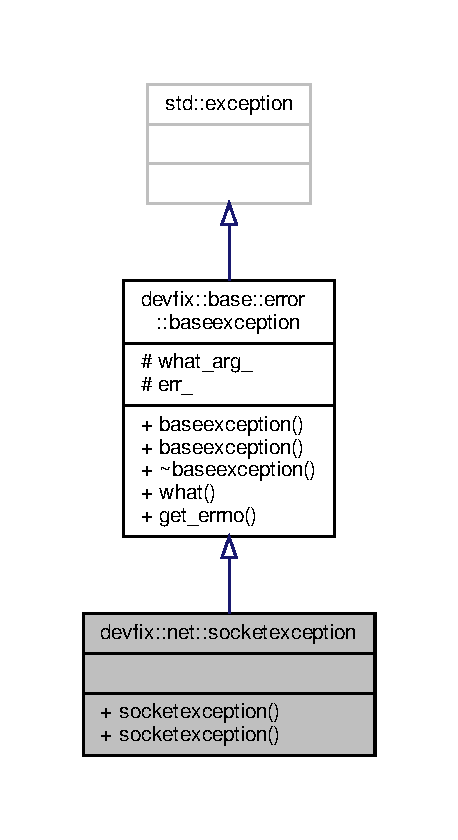
\includegraphics[width=220pt]{structdevfix_1_1net_1_1socketexception__inherit__graph}
\end{center}
\end{figure}
\subsection*{Public Member Functions}
\begin{DoxyCompactItemize}
\item 
\hyperlink{structdevfix_1_1net_1_1socketexception_aeab5d004d494103b37156a5f23a5296a}{socketexception} (const std\+::string \&what\+\_\+arg, int err=-\/1)
\item 
\hyperlink{structdevfix_1_1net_1_1socketexception_a6da69f635eb11f932a0e960545d023bd}{socketexception} (const char $\ast$what\+\_\+arg, int err=-\/1)
\end{DoxyCompactItemize}
\subsection*{Additional Inherited Members}


\subsection{Detailed Description}
Thrown to indicate that there is an error creating or accessing a Socket. 

\subsection{Constructor \& Destructor Documentation}
\mbox{\Hypertarget{structdevfix_1_1net_1_1socketexception_aeab5d004d494103b37156a5f23a5296a}\label{structdevfix_1_1net_1_1socketexception_aeab5d004d494103b37156a5f23a5296a}} 
\index{devfix\+::net\+::socketexception@{devfix\+::net\+::socketexception}!socketexception@{socketexception}}
\index{socketexception@{socketexception}!devfix\+::net\+::socketexception@{devfix\+::net\+::socketexception}}
\subsubsection{\texorpdfstring{socketexception()}{socketexception()}\hspace{0.1cm}{\footnotesize\ttfamily [1/2]}}
{\footnotesize\ttfamily devfix\+::net\+::socketexception\+::socketexception (\begin{DoxyParamCaption}\item[{const std\+::string \&}]{what\+\_\+arg,  }\item[{int}]{err = {\ttfamily -\/1} }\end{DoxyParamCaption})\hspace{0.3cm}{\ttfamily [inline]}, {\ttfamily [explicit]}}

Constructs the error object with what\+\_\+arg as explanatory string that can be accessed through \hyperlink{structdevfix_1_1base_1_1error_1_1baseexception_a16327152a55d65b1e537825231fbd452}{what()}. 
\begin{DoxyParams}{Parameters}
{\em what\+\_\+arg} & explanatory std\+::string \\
\hline
{\em err} & c error code (errno) \\
\hline
\end{DoxyParams}
\mbox{\Hypertarget{structdevfix_1_1net_1_1socketexception_a6da69f635eb11f932a0e960545d023bd}\label{structdevfix_1_1net_1_1socketexception_a6da69f635eb11f932a0e960545d023bd}} 
\index{devfix\+::net\+::socketexception@{devfix\+::net\+::socketexception}!socketexception@{socketexception}}
\index{socketexception@{socketexception}!devfix\+::net\+::socketexception@{devfix\+::net\+::socketexception}}
\subsubsection{\texorpdfstring{socketexception()}{socketexception()}\hspace{0.1cm}{\footnotesize\ttfamily [2/2]}}
{\footnotesize\ttfamily devfix\+::net\+::socketexception\+::socketexception (\begin{DoxyParamCaption}\item[{const char $\ast$}]{what\+\_\+arg,  }\item[{int}]{err = {\ttfamily -\/1} }\end{DoxyParamCaption})\hspace{0.3cm}{\ttfamily [inline]}, {\ttfamily [explicit]}}

Constructs the error object with what\+\_\+arg as explanatory string that can be accessed through \hyperlink{structdevfix_1_1base_1_1error_1_1baseexception_a16327152a55d65b1e537825231fbd452}{what()}. 
\begin{DoxyParams}{Parameters}
{\em what\+\_\+arg} & explanatory c-\/string \\
\hline
{\em err} & c error code (errno) \\
\hline
\end{DoxyParams}


The documentation for this struct was generated from the following file\+:\begin{DoxyCompactItemize}
\item 
devfix/net/\hyperlink{socketexception_8h}{socketexception.\+h}\end{DoxyCompactItemize}

\hypertarget{structdevfix_1_1base_1_1timeoutexception}{}\section{devfix\+:\+:base\+:\+:timeoutexception Struct Reference}
\label{structdevfix_1_1base_1_1timeoutexception}\index{devfix\+::base\+::timeoutexception@{devfix\+::base\+::timeoutexception}}


{\ttfamily \#include $<$timeoutexception.\+h$>$}



Inheritance diagram for devfix\+:\+:base\+:\+:timeoutexception\+:
% FIG 0


Collaboration diagram for devfix\+:\+:base\+:\+:timeoutexception\+:
% FIG 1
\subsection*{Public Member Functions}
\begin{DoxyCompactItemize}
\item 
\hyperlink{structdevfix_1_1base_1_1timeoutexception_ad900adf164c04e3a33dafd38ded1f024}{timeoutexception} (const std\+::string \&what\+\_\+arg, int err=-\/1)
\item 
\hyperlink{structdevfix_1_1base_1_1timeoutexception_a684cb2e6e0d78b98d30c505a6bf9066d}{timeoutexception} (const char $\ast$what\+\_\+arg, int err=-\/1)
\end{DoxyCompactItemize}
\subsection*{Additional Inherited Members}


\subsection{Detailed Description}
Exception for timeouts. 
\begin{DoxyTemplParams}{Template Parameters}
{\em T} & Type of character \\
\hline
\end{DoxyTemplParams}


\subsection{Constructor \& Destructor Documentation}
\mbox{\Hypertarget{structdevfix_1_1base_1_1timeoutexception_ad900adf164c04e3a33dafd38ded1f024}\label{structdevfix_1_1base_1_1timeoutexception_ad900adf164c04e3a33dafd38ded1f024}} 
\index{devfix\+::base\+::timeoutexception@{devfix\+::base\+::timeoutexception}!timeoutexception@{timeoutexception}}
\index{timeoutexception@{timeoutexception}!devfix\+::base\+::timeoutexception@{devfix\+::base\+::timeoutexception}}
\subsubsection{\texorpdfstring{timeoutexception()}{timeoutexception()}\hspace{0.1cm}{\footnotesize\ttfamily [1/2]}}
{\footnotesize\ttfamily devfix\+::base\+::timeoutexception\+::timeoutexception (\begin{DoxyParamCaption}\item[{const std\+::string \&}]{what\+\_\+arg,  }\item[{int}]{err = {\ttfamily -\/1} }\end{DoxyParamCaption})\hspace{0.3cm}{\ttfamily [inline]}, {\ttfamily [explicit]}}

Constructs the exception object with what\+\_\+arg as explanatory std\+::string that can be accessed through \hyperlink{structdevfix_1_1base_1_1exception_ad2066a6a81737c0fdf776120a6ca69d2}{what()}. 
\begin{DoxyParams}{Parameters}
{\em what\+\_\+arg} & description \\
\hline
\end{DoxyParams}
\mbox{\Hypertarget{structdevfix_1_1base_1_1timeoutexception_a684cb2e6e0d78b98d30c505a6bf9066d}\label{structdevfix_1_1base_1_1timeoutexception_a684cb2e6e0d78b98d30c505a6bf9066d}} 
\index{devfix\+::base\+::timeoutexception@{devfix\+::base\+::timeoutexception}!timeoutexception@{timeoutexception}}
\index{timeoutexception@{timeoutexception}!devfix\+::base\+::timeoutexception@{devfix\+::base\+::timeoutexception}}
\subsubsection{\texorpdfstring{timeoutexception()}{timeoutexception()}\hspace{0.1cm}{\footnotesize\ttfamily [2/2]}}
{\footnotesize\ttfamily devfix\+::base\+::timeoutexception\+::timeoutexception (\begin{DoxyParamCaption}\item[{const char $\ast$}]{what\+\_\+arg,  }\item[{int}]{err = {\ttfamily -\/1} }\end{DoxyParamCaption})\hspace{0.3cm}{\ttfamily [inline]}, {\ttfamily [explicit]}}

Constructs the exception object with what\+\_\+arg as explanatory c-\/string that can be accessed through \hyperlink{structdevfix_1_1base_1_1exception_ad2066a6a81737c0fdf776120a6ca69d2}{what()}. 
\begin{DoxyParams}{Parameters}
{\em what\+\_\+arg} & description \\
\hline
\end{DoxyParams}


The documentation for this struct was generated from the following file\+:\begin{DoxyCompactItemize}
\item 
devfix/base/timeoutexception.\+h\end{DoxyCompactItemize}

%--- End generated contents ---

% Index
\backmatter
\newpage
\phantomsection
\clearemptydoublepage
\addcontentsline{toc}{chapter}{Index}
\printindex

\end{document}
